\documentclass{jarticle}

\usepackage{graphicx}
\usepackage{url}
\usepackage{listings,jlisting}
\usepackage{ascmac}
\usepackage{amsmath,amssymb}

%ここからソースコードの表示に関する設定
\lstset{
  basicstyle={\ttfamily},
  identifierstyle={\small},
  commentstyle={\smallitshape},
  keywordstyle={\small\bfseries},
  ndkeywordstyle={\small},
  stringstyle={\small\ttfamily},
  frame={tb},
  breaklines=true,
  columns=[l]{fullflexible},
  numbers=left,
  xrightmargin=0zw,
  xleftmargin=3zw,
  numberstyle={\scriptsize},
  stepnumber=1,
  numbersep=1zw,
  lineskip=-0.5ex
}
%ここまでソースコードの表示に関する設定 

\title{知能プログラミング演習II 課題1}
\author{グループ07\\
  29114007 池口 弘尚\\
  29114031 大原 拓人\\
  29114048 北原 太一\\
  29114086 飛世 裕貴\\
  29114095 野竹 浩二朗\\
%  {\small (グループレポートの場合は、グループ名および全員の学生番号と氏名が必要)}
}
\date{2019年10月7日}

\begin{document}
\maketitle

\paragraph{提出物} rep1 group07.zip
\paragraph{グループ} グループ07

\section{課題の説明}
\begin{description}
  \item[課題1-1] Search.javaの状態空間におけるパラメータ(コストや評価値)を様々に変化させて実行し,
        各探索手法の違いを説明せよ.
        具体的には,変化させたパラメータと探索結果(最短パス探索の成否,
        解を返すまでのステップ数,etc.)の関係を,探索手法毎に表やグラフ等にまとめよ.
        それらの結果を参照して考察を行い,各探索手法の違いを説明せよ.
  \item[課題1-2] グループでの進捗管理や成果物共有などについて,工夫した点や使ったツールについて考察せよ.
  \item[課題1-3] Search.javaの探索過程や最終的に得られた順路をユーザに視覚的に示すGUIを作成せよ.
\end{description}


\section{課題1-1}
\begin{screen}
  Search.javaの状態空間におけるパラメータ(コストや評価値)を様々に変化させて実行し,
  各探索手法の違いを説明せよ.
  具体的には,変化させたパラメータと探索結果(最短パス探索の成否,
  解を返すまでのステップ数,etc.)の関係を,探索手法毎に表やグラフ等にまとめよ.
  それらの結果を参照して考察を行い,各探索手法の違いを説明せよ.
\end{screen}
\subsection{手法}
課題で与えられた探索手法と、我々が考察した点は以下のとおりである。

\begin{enumerate}
  \item 幅優先探索法
  \item 深さ優先探索法
  \item 分枝限定法
  \item 山登り法
  \item 最良優先探索法
  \item A*アルゴリズム
\end{enumerate}

各探索法について、状態空間のパラメータを手動で変更して無限ループに
陥らせたり、ステップ数の増減を観察した。またパラメータをRandomクラス
を用いて変動させ試行を繰り返し、最小コストでゴールにたどり着ける手法を
探した。
\subsection{実装}

もともと与えられたSearch.javaを以下のように変更した。

\paragraph{}
状態空間のパラメータをRandomクラスで変動させられるように、
地点名、ヒューリスティック関数、
各エッジのコストと、出発元と行先の番号を配列に保存するようにした。
また、手法ごとに同じパラメータで探索が行えるように、
保存した配列をもとに状態空間をリセットできるようにした。
その仕様により、それぞれの状態空間ごとに最小のコストでゴールに
たどり着ける探索手法とその時のステップ数を比較できるようになった。\\

\paragraph{}
地点名、ヒューリスティック関数、各エッジのコストと、
出発元と行先の番号を配列に保存するようにした
部分と、それをもとに状態空間を生成する部分を
抜粋したコードは以下のとおりである。

\begin{lstlisting}[caption=SearchRandクラスより抜粋]
  // ノード名
	String[] locations = { "L.A.Airport", "UCLA", "Hoolywood", "Anaheim", "GrandCanyon", "SanDiego", "Downtown",
			"Pasadena", "DisneyLand", "Las Vegas" };
	// 分岐元のインデックス
	int[] nodeIndex = { 0, 0, 1, 1, 2, 2, 2, 3, 3, 3, 4, 4, 5, 6, 6, 7, 7, 8 };
	// 分岐先のインデックス
	int[] childIndex = { 1, 2, 2, 6, 3, 6, 7, 4, 7, 8, 8, 9, 1, 5, 7, 8, 9, 9 };
	int[] nodeRand;
	int[] costRand;
	int randSize = 99;
	// N回試行の記録(Method,0.step 1.cost)
  int[][] record = new int[2][6];
  public int[][] getRecord() {
    return record;
  }
  SearchRand() {
    // コストとヒューリスティック関数の決定
    Random rand = new Random();
    nodeRand = new int[10];
    costRand = new int[18];
    for (int i = 0; i < nodeRand.length; i++) {
      if (i != 0 && i != nodeRand.length - 1)
        nodeRand[i] = rand.nextInt(randSize) + 1;
      else
        nodeRand[i] = 0;
    }
    for (int i = 0; i < costRand.length; i++)
      costRand[i] = rand.nextInt(randSize) + 1;
    makeStateSpace();
  }
  
  private void makeStateSpace() {
    // 状態空間の生成
    NodeRand[] nodelist = new NodeRand[10];
    for (int i = 0; i < locations.length; i++)
      nodelist[i] = new NodeRand(locations[i], nodeRand[i]);
    for (int i = 0; i < nodeIndex.length; i++)
      nodelist[nodeIndex[i]].addChild(nodelist[childIndex[i]], costRand[i]);
    node = nodelist.clone();
    start = node[0];
    goal = node[9];
  }
\end{lstlisting}

\paragraph{}
各手法で見つけた経路のコストと、それまでにかかったステップ数を配列に保存し、
すべての手法の探索が終わった後にその結果を比較する実装は以下のとおりである。

\begin{lstlisting}[caption=結果を保存し、比較]
	public final int hillClimbing = 3;
  ...
  if (success) {
			// System.out.println("*** Solution ***");
			// printSolution(goal, step);
			record[STEP][hillClimbing] = step;
			record[COST][hillClimbing] = goal.getGValue();
		} else {
			//System.out.println("faild\nstep:" + step);
			record[STEP][hillClimbing] = step;
			record[COST][hillClimbing] = step * (randSize + 1);
		}
  ...
  // 同じ状態空間で探索を行った後
  int[][] record = place.getRecord();
  int minCost = getMin(record[1]);// 6手法中の最小コスト
  for (int j = 0; j < record[1].length; j++) {
    if (minCost == record[1][j]) {
      //最小コストのときカウント
      counts[1][j]++;
      //分枝限定法よりA*アルゴリズムのステップ数が多いとき
      //分枝限定法よりステップ数が少ないか
      if(record[0][2]<record[0][5]){
        if(record[0][j]<=record[0][2])
          counts[0][j]++;
      }else{
        //A*アルゴリズムよりステップ数が少ないか
        if(record[0][j]<=record[0][5])
          counts[0][j]++;
        }
      }
    }
  if(record[0][3]==100)hillloop++;

\end{lstlisting}

\subsection{実行例}
ランダムに状態空間のパラメータを1から9の間で変更した試行を繰り返し、最短経路を
発見した回数と、より少ないステップ数で最短経路を発見した回数は以下のとおりである。
入れ替わっているが、counts[0]は後者、counts[1]は前者である。
山登り法が無限ループに陥った回数もカウントした。

\begin{lstlisting}
  counts[0][0]:206679,counts[1][0]:471074
  counts[0][1]:110876,counts[1][1]:122587
  counts[0][2]:203326,counts[1][2]:1000000
  counts[0][3]:106402,counts[1][3]:106436
  counts[0][4]:213036,counts[1][4]:251926
  counts[0][5]:802176,counts[1][5]:848311
  hillloop:298951
  counts[0][0]:207610,counts[1][0]:471056
  counts[0][1]:111085,counts[1][1]:122867
  counts[0][2]:202782,counts[1][2]:1000000
  counts[0][3]:106586,counts[1][3]:106610
  counts[0][4]:213300,counts[1][4]:251970
  counts[0][5]:803118,counts[1][5]:848982
  hillloop:298163
\end{lstlisting}

ランダムに状態空間のパラメータを1から99の間で変更した場合は以下のようになった。

\begin{lstlisting}
  counts[0][0]:13493,counts[1][0]:37236
  counts[0][1]:8747,counts[1][1]:10424
  counts[0][2]:27577,counts[1][2]:100000
  counts[0][3]:10212,counts[1][3]:10215
  counts[0][4]:16967,counts[1][4]:20453
  counts[0][5]:69439,counts[1][5]:77482
  hillloop:28461
  counts[0][0]:13318,counts[1][0]:36973
  counts[0][1]:8827,counts[1][1]:10537
  counts[0][2]:27631,counts[1][2]:100000
  counts[0][3]:10231,counts[1][3]:10235
  counts[0][4]:17010,counts[1][4]:20508
  counts[0][5]:69210,counts[1][5]:77383
  hillloop:28604
\end{lstlisting}

分枝限定法が必ず最短経路を見つけていることがわかる。

\subsection{考察}
A*アルゴリズムは必ず最短経路を発見できると勘違いしていたが、
ヒューリスティック関数が影響して最短経路ではない経路を発見して
終了する場合があることがわかった。
もともと、状態空間のノードのつなぎ方は変動していないので
条件としてはかなり限定されているが、A*アルゴリズムが最短経路を
発見したときは分枝限定法より少ないステップ数で発見できている。
また、山登り法が無限ループに陥る確率もある程度収束しているように思われる。
\paragraph{}
手動で状態空間のパラメータを変更した際の考察については、
グループレポートを参考にされたい。

\subsection{実装}
与えられたSearch.javaにおいて、2. 4. 5.の手法を用いると、無限ループに陥ってしまう状態空間を作成した。
\begin{figure}[htbp]
  \centering
  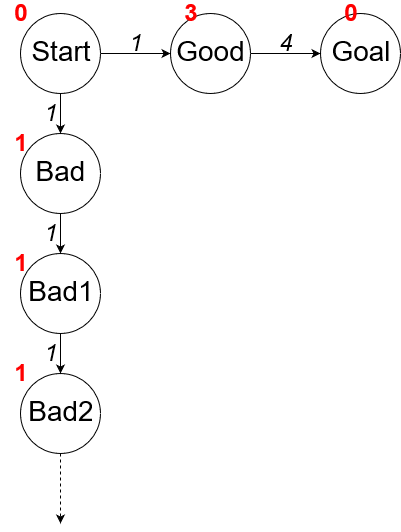
\includegraphics[bb=0 0 401 532,width=0.6\linewidth]{Infinite.png}
  \caption{無限ループに陥る状態空間}
\end{figure}


深さ優先探索法に関して、反復深化深さ優先探索とすることにより、先述の状態空間においても解を求めることができるようにした。
\subsubsection{BadNode}

まず、このクラスは、与えられたNodeクラスのサブクラスである。
オーバーライドしたメソッドは以下の1つ。
\begin{itemize}
  \item getChildren: Nodeクラスでは内部メンバchildrenを返すが、BadNodeでは新しいBadNodeインスタンスをaddChildしてからchildrenを返す。

\end{itemize}

BadNodeクラスの実装を以下に示す。
\begin{lstlisting}[caption=BadNodeクラス,label=src:BadNode]
      //無限ループを形成するノード
      class BadNode extends Node {
  
          static int id = 0; //名付け用ID
          BadNode(String theName, int theHValue) {
              super(theName, theHValue);
          }
  
          @Override
          public ArrayList<Node> getChildren() {
              addChild(new BadNode("Bad" + ++id, hValue), 1); //新しいBadNodeをchildrenに追加
              return super.getChildren(); //childrenを返す
          }
      }
  \end{lstlisting}

\subsubsection{深さ優先探索}
深さ優先探索をするdepthFirstメソッドを、以下のように改良した。
\begin{lstlisting}[caption=depthFirstメソッド,label=src:depthFirst]
  /***
    * 反復深化深さ優先探索
    */
  public void depthFirst() {
    ArrayList<Node> open = new ArrayList<Node>();
    open.add(start);
    ArrayList<Node> newOpen = new ArrayList<>(); //深さが1レベル深いオープンリスト
    ArrayList<Node> closed = new ArrayList<Node>();
    boolean success = false;
    int step = 0;

    for (;;) {
      System.out.println("STEP:" + (step++));
      System.out.println("OPEN:" + open.toString());
      System.out.println("NEWOPEN:" + newOpen.toString());
      System.out.println("CLOSED:" + closed.toString());
      // openは空か?
      if (open.size() == 0) {
        //newOpenも空か?
        if (newOpen.size() == 0) {
            success = false;
            break;
        }
        //探索を1レベル深くし、newOpenをリセット
        open = newOpen;
        newOpen = new ArrayList<>();
      } else {
        // openの先頭を取り出し node とする.
        Node node = open.get(0);
        open.remove(0);
        // node は ゴールか?
        if (node == goal) {
            success = true;
            break;
        } else {
        // node を展開して子節点をすべて求める.
        ArrayList<Node> children = node.getChildren();
        // node を closed に入れる.
        closed.add(node);
        // 子節点 m が open にも newOpen にも closed にも含まれていなければ,
        // 以下を実行.幅優先探索と異なるのはこの部分である.
        // j は複数の子節点を適切にnewOpenの先頭に置くために位置
        // を調整する変数であり,一般には展開したときの子節点
        // の位置は任意でかまわない.
        int j = 0;
        for (int i = 0; i < children.size(); i++) {
          Node m = children.get(i);
          if (!open.contains(m) && !newOpen.contains(m) && !closed.contains(m)) {
            // m から node へのポインタを付ける
            m.setPointer(node);
            //newOpenに追加
            if (m == goal) {
                newOpen.add(0, m);
            } else {
                newOpen.add(j, m);
            }
            j++;
          }
        }
        }
      }
    }
    if (success) {
        System.out.println("*** Solution ***");
        printSolution(goal);
    }
  }
  
  \end{lstlisting}

\subsection{実行例}
BadNodeを用いた状態空間に対し、深さ優先探索、反復深化深さ優先探索、山登り法を実行した結果を以下に示す。

\begin{lstlisting}[caption=深さ優先探索]
  (前略)
  STEP:848
  OPEN:[Bad846(h:1), Good(h:3)]
  CLOSED:[Start(h:0), Bad(h:1), Bad0(h:1), Bad1(h:1), Bad2(h:1), (中略), Bad843(h:1), Bad844(h:1), Bad845(h:1)]
  STEP:849
  OPEN:[Bad847(h:1), Good(h:3)]
  CLOSED:[Start(h:0), Bad(h:1), Bad0(h:1), Bad1(h:1), Bad2(h:1), (中略), Bad844(h:1), Bad845(h:1), Bad846(h:1)]
  STEP:850
  (以下略)
  \end{lstlisting}

\begin{lstlisting}[caption=反復深化深さ優先探索]
  Depth First Search
  STEP:0
  OPEN:[Start(h:0)]
  NEWOPEN:[]
  CLOSED:[]
  STEP:1
  OPEN:[]
  NEWOPEN:[Bad(h:1), Good(h:3)]
  CLOSED:[Start(h:0)]
  STEP:2
  OPEN:[Bad(h:1), Good(h:3)]
  NEWOPEN:[]
  CLOSED:[Start(h:0)]
  STEP:3
  OPEN:[Good(h:3)]
  NEWOPEN:[Bad0(h:1)]
  CLOSED:[Start(h:0), Bad(h:1)]
  STEP:4
  OPEN:[]
  NEWOPEN:[Goal(h:0), Bad0(h:1)]
  CLOSED:[Start(h:0), Bad(h:1), Good(h:3)]
  STEP:5
  OPEN:[Goal(h:0), Bad0(h:1)]
  NEWOPEN:[]
  CLOSED:[Start(h:0), Bad(h:1), Good(h:3)]
  *** Solution ***
  Goal(h:0) <- Good(h:3) <- Start(h:0)
  \end{lstlisting}

\begin{lstlisting}[caption=山登り法]
  (前略)
  [Bad199906(h:1)]
  [Bad199907(h:1)]
  [Bad199908(h:1)]
  [Bad199909(h:1)]
  (以下略)
  \end{lstlisting}

\subsection{考察}
深さ優先探索、山登り法の場合、解(Goal)のほうに進むGoodノード
には進まず、解が存在しないがヒューリスティクス関数がより良い
Badノードに進んでしまう。しかしながら、反復進化深さ優先探索
により、探索するノードの深さを制限することにより、深さ優先探索
で探索できない状態空間でも解を求めることができる。

\subsection{実装}
今回の課題ではプログラム自体は変えずに、
状態空間のパラメータのみを変化させた。
\subsection{実行例}

まず、パラメータに変更を加える前の各探索手法におけるSTEP数
と探索結果を以下に示す。
\begin{table}[h]
  \begin{tabular}{|l|c|l|}
    \hline
    探索手法       & \multicolumn{1}{l|}{STEP数} & 探索結果                                                                                                                 \\ \hline
    幅優先探索     & 7                           & LasVegas \textless{}- Pasadena \textless{}- Hoolywood \textless{}- L.A.Airport                                           \\ \hline
    深さ優先探索   & 6                           & LasVegas \textless{}- Pasadena \textless{}- Downtown \textless{}- UCLA \textless{}- L.A.Airport                          \\ \hline
    分岐限定法     & 8                           & LasVegas \textless{}- DisneyLand \textless{}- Pasadena \textless{}- Hoolywood \textless{}- UCLA \textless{}- L.A.Airport \\ \hline
    山登り法       & -                           & 探索失敗                                                                                                                 \\ \hline
    最良優先探索   & 6                           & LasVegas \textless{}- Pasadena \textless{}- Hoolywood \textless{}- L.A.Airport                                           \\ \hline
    A*アルゴリズム & 8                           & LasVegas \textless{}- DisneyLand \textless{}- Pasadena \textless{}- Hoolywood \textless{}- UCLA \textless{}- L.A.Airport \\ \hline
  \end{tabular}
\end{table}

この結果より山登り法において探索が失敗していることがわかる。
これはあるノードにおいて次のノードのヒューリスティックスの値のみ
で探索をしていく山登り法ではUCLA、Downtown、Sandiegoにおいて
無限ループが生じるためである。以下では、分枝限定法に関しては
STEP数をより小さく、山登り法に関しては探索が成功するように
パラメータを変更していく。なお、今回のプログラムにおいて
幅優先探索と深さ優先探索ではコストやヒューリスティックス
の値は考慮しておらず、パラメータの変更が影響を及ぼさないため、
記述は省略する。

まず、分枝限定法における探索STEP数を小さくするために、
UCLAからDowntownへのコストを11、HoolywoodからAnaheim・
Downtownへのコストを10とした。この時の結果を以下に示す。


\begin{table}[ht]
  \begin{tabular}{|l|c|l|}
    \hline
    探索手法       & \multicolumn{1}{l|}{STEP数} & 探索結果                                                                                                                 \\ \hline
    分岐限定法     & 6                           & LasVegas \textless{}- DisneyLand\textless{}- Pasadena \textless{}- Hoolywood \textless{}- UCLA \textless{}- L.A.Airport  \\ \hline
    山登り法       & -                           & 探索失敗                                                                                                                 \\ \hline
    最良優先探索   & 6                           & LasVegas \textless{}- Pasadena \textless{}- Hoolywood \textless{}- L.A.Airport                                           \\ \hline
    A*アルゴリズム & 7                           & LasVegas \textless{}- DisneyLand \textless{}- Pasadena \textless{}- Hoolywood \textless{}- UCLA \textless{}- L.A.Airport \\ \hline
  \end{tabular}
\end{table}

この変更においてA*アルゴリズムが最短経路を発見することは保障されているため、分枝限定法によって最短経路を最小STEP数で探索されていることがわかる。

次に山登り法による探索を成功させるために初期パラメータから、Sandiegoのヒューリスティックスの値を5に変更した。この時の結果を以下に示す。

\begin{table}[ht]
  \begin{tabular}{|l|c|l|}
    \hline
    探索手法       & \multicolumn{1}{l|}{STEP数} & 探索結果                                                                                                                 \\ \hline
    分岐限定法     & 8                           & LasVegas \textless{}- DisneyLand \textless{}- Pasadena \textless{}- Hoolywood \textless{}- UCLA \textless{}- L.A.Airport \\ \hline
    山登り法       & 5                           & LasVegas \textless{}- Pasadena \textless{}- Downtown \textless{}- Hoolywood  \textless{}- L.A.Airport                    \\ \hline
    最良優先探索   & 5                           & LasVegas \textless{}- Pasadena \textless{}- Hoolywood \textless{}- L.A.Airport                                           \\ \hline
    A*アルゴリズム & 8                           & LasVegas \textless{}- DisneyLand \textless{}- Pasadena \textless{}- Hoolywood \textless{}- UCLA \textless{}- L.A.Airport \\ \hline
  \end{tabular}
\end{table}

この結果から変更によって山登り法による探索が成功することが
確認できた。しかしこの変更においてもA*アルゴリズムが最短経路
を発見することは保証されているため、山登り法により最短経路が
探索されていないことがわかる。
\subsection{考察}

本課題において分枝限定法に関して上記のように、
変更を行った結果探索STEP数を小さくすることができた。
その理由として、初期値においては最短経路には含まれない
Downtownへの探索を行っており、変更によってその余分な処理
を省くことができたからだと考えられる。

また、分枝限定法と同様にA*アルゴリズムでも最短経路の探索
に成功しているが、STEP数に関しては分枝限定法の方が小さくなっている。
今回のように経路のパラメータによっては、無駄な処理を省略する
分枝限定法の方が探索を早く終えることができる。

そして山登り法に関しては、今回のプログラムにおいて繰り返し回避
のための工夫がなされていないため、初期値のように正しくパラメータ
を設定していなければ無限ループを起こしてしまう。またゴールノード
を子ノードに持つノードに到達すると、最もヒューリスティックスの
値が小さいノードがゴールノードとなってしまい、ゴールまでのコスト
に関係なくゴールへ探索を進めてしまう。今回の変更後の探索において、
最短経路探索のためにはゴールノードを子ノードに持つPasadenaを
経由しなければならないため、正しく最短経路が探索できなかったと
考えられる。そのため、今回の経路探索において山登り法により正しい
最短経路を求めるにはPasadenaからLasVegasへのコストを小さくする
必要があったと考えられる。また今回はプログラム自体への変更を行わず
にパラメータを変更することで無限ループに陥ることを防いだが、
繰り返し探索を防止することで無限ループを防ぐことができると考える。

\subsection{実装}
プログラムのコード本体は変えず、状態空間のパラメータのみを変化させた。

\subsection{実行例}
幅優先探索、深さ優先探索については、パラメータを変化させても結果
は変わらないため、省略する。また、実行結果すべてを載せてしまうと
無駄に長くなってしまうため、STEP数と採取的にどのルートになったか
のみを記す。

まず、最良優先が成功する場合として、コスト、評価値を変化させた。
\begin{table}[h]
  \begin{tabular}{|l|c|l|}
    \hline
    探索手法       & \multicolumn{1}{l|}{STEP数} & 探索結果                                                                                         \\ \hline
    分岐限定法     & 7                           & LasVegas \textless{}- Pasadena \textless{}- Hoolywood \textless{}- L.A.Airport                   \\ \hline
    山登り法       & -                           & LasVegas \textless{}- Pasadena \textless{}- Hoolywood \textless{}- UCLA \textless{}- L.A.Airport \\ \hline
    最良優先探索   & 4                           & LasVegas \textless{}- Pasadena \textless{}- Hoolywood \textless{}- L.A.Airport                   \\ \hline
    A*アルゴリズム & 5                           & LasVegas \textless{}- Pasadena \textless{}- Hoolywood \textless{}- L.A.Airport                   \\ \hline
  \end{tabular}
\end{table}
分岐限定法、最良優先探索、A*アルゴリズムが成功していることが分かる。\\
ステップ数を比較すると、最良優先探索が少なく、分岐限定法が多くなっている。
最良優先探索が上手くいくようにパラメータを調整したので、そのステップ数が少なく
なることは当然である。\\

次に、A*アルゴリズムが失敗するようにPasadenaの評価値を10とした。
\begin{table}[ht]
  \begin{tabular}{|l|c|l|}
    \hline
    探索手法       & \multicolumn{1}{l|}{STEP数} & 探索結果                                                                                                                 \\ \hline
    分岐限定法     & 7                           & LasVegas \textless{}- DisneyLand\textless{}- Pasadena \textless{}- Hoolywood \textless{}- UCLA \textless{}- L.A.Airport  \\ \hline
    山登り法       & -                           & \multicolumn{1}{c|}{-}                                                                                                   \\ \hline
    最良優先探索   & 6                           & LasVegas \textless{}- GrandCanyon \textless{}- Anaheim \textless{}- Hoolywood \textless{}- L.A.Airport                   \\ \hline
    A*アルゴリズム & 5                           & LasVegas \textless{}- GrandCanyon \textless{}- Anaheim \textless{}- Hoolywood \textless{}- UCLA \textless{}- L.A.Airport \\ \hline
  \end{tabular}
\end{table}
分岐限定法は成功しているが、山登り法は無限ループ、
最良優先探索とA*アルゴリズムはゴールに到達しているものの、
最短のルートではなかった。
\subsection{考察}
最良優先探索の場合、ゴールノードを子ノードに持つノードに
たどり着くと、そこからゴールまでのコストに関係なくゴールへと
行ってしまう。今回の場合、初期のパラメータだとPasadenaからは
一度DisneyLandを経由しなければならないが、最良優先探索では
それができないので、成功する例として、コストを無理やり減らす
ということをしなければならなかった。実際は、コストを変えること
は難しいため、ヒューリスティックスのみでは不十分であることが分かる。\\
A*アルゴリズムは、ヒューリスティックスに加えて、
コストも考慮することができるため、最良優先探索では
成功できない場合でもしっかりと探索することができる。
しかし、ヒューリスティックスに加えて、コストも見なければ
ならないのでステップ数は増えてしまっている。


\section{課題1-2}
\begin{screen}
  グループでの進捗管理や成果物共有などについて,
  工夫した点や使ったツールについて考察せよ.
\end{screen}

課題1-2は実装を伴わない課題であるため、考察のみ記す。

\subsection{考察}
  今回は、扱っているデータがそれほど機密性の高いものではなかったため、
  連絡の手段としてはより気軽に使えることを重視して、LINE を使用した。普
  段から使っているツールを使用することによって、より円滑なコミュニケー
  ションを図った。しかし、それぞれのメンバーが進捗を報告しているわけでは
  なかったので、どれだけ進捗しているのかわからないという状況になってし
  まった。そのため、進捗管理にはどれだけ進んでいるのかなどがわかる Trello
  なども活用していくことが重要だと思う。成果物共有に関しては、git を使
  用した。git を使ったことがないメンバーが多かったので、今回はプルとプッ
  シュのみで作業を行った。そのためにそれぞれの作業をフォルダごとに分け
  て管理した。今回の課題では、あまりソースコードを変える必要がなかった
  ためできたことだが、次回の課題からはソースコードを書くことになると思
  うので、ブランチを分けて作業していく必要があると考える。

\subsection{考察}
  今回は課題の分量が少なかったので、演習時間内に終わらなかった分は
  後日全員で集まって課題を進めた。
  連絡手段としてLINEを用いた。今後の予定としては、
  GitHubを用いて進捗状況の共有をできるようにしたい。
\subsection{考察}
  演習時間内に終わらなかった分は後日全員で集まって課題を進めた。
  連絡手段としてLINEを、ファイル管理にGitHubを用いた。
\subsection{考察}
  事務連絡についてはLINEを用いた。ファイルはGitHubを用いて共有した。
  LINEに関しては、ずっと使っているものなので特に不便を感じることは無かった。
  GitHubはファイルの共有するため、初めて使った。まだまだ機能についてあまり分かっていないので少しずつ使いこなせるようにしていきたい。

\section{課題1-3}
\begin{screen}
  Search.javaの探索過程や最終的に得られた順路をユーザに視覚的に示すGUIを作成せよ.
\end{screen}
\subsection{実装}
まず、新たに追加したクラスは以下の
\begin{itemize}
  \item DrawArrowクラス: Path2D.Floatを継承。向きがある矢印の描画をするためのクラスであり、参考文献のコードを利用した。
  \item FrameBaseクラス: JFrameを継承。コンストラクタのみ実装しており、JFrameの各種設定が1行でできるようにしてある。
  \item GraphPanelクラス: JPanelを継承。各種グラフを描画するためのメソッドが実装されている。
  \item MakeGUIクラス: 各種GUIを作成するためのクラス。
\end{itemize}

DrawArrowクラスについては参考文献\cite{goo}をそのまま用いた。

FrameBaseクラスでは、JFrameのサイズやウィンドウを閉じたときにプログラムを終了
することなどを一括して設定するためのコンストラクタを以下のように実装した。

\begin{lstlisting}[caption=FrameBaseのコンストラクタ,label=src:FrameBase]
	//位置を指定
    public FrameBase(String title,int x,int y,int width,int height) {
		setTitle(title);
		setBounds(x, y, width, height);
		setDefaultCloseOperation(JFrame.EXIT_ON_CLOSE);
	}
	//中央に表示
	public FrameBase(String title,int width,int height) {
		setTitle(title);
		setSize(width, height);
		setLocationRelativeTo(null);
		setDefaultCloseOperation(JFrame.EXIT_ON_CLOSE);
	}
\end{lstlisting}

GraphPanelクラスでは、探索のグラフを表示するための様々なメソッドが実装してある。
探索木を表示することに関連するmakeTreeList,addTreeList,selectTreeNode,
removeNodeFromTree,addLeaf,addGoalは以下のように実装した。
\begin{lstlisting}[caption=探索木関連のメソッド,label=src:MakeGUI1]
	//ルートノードを作成
	public void makeTreeList(Node root) {
		nodeMap = new HashMap<>();
		//clear();
		DefaultMutableTreeNode rootNode = new DefaultMutableTreeNode(root);
		nodeMap.put(root.name, rootNode);
		tree = new JTree(rootNode);
		add(tree);
		setVisible(false);
		setVisible(true);
	}
	//pをcの親にする
	public void addTreeList(Node p, Node c) {
		DefaultMutableTreeNode parent = nodeMap.get(p.name);
		if (parent == null) {
			System.out.println("error");
			return;
		}
		DefaultMutableTreeNode child = new DefaultMutableTreeNode(c);
		parent.add(child);
		nodeMap.put(c.name, child);
		DefaultTreeModel m = (DefaultTreeModel) tree.getModel();
		m.reload();
		for (int i = 0; i < tree.getRowCount(); i++) {
			tree.expandRow(i);
		}
	}
	
    //nodeを選択状態にする
	public void selectTreeNode(Node node) {
		DefaultMutableTreeNode p = nodeMap.get(node.name);
		tree.setSelectionPath(new TreePath(p.getPath()));
	}

	//cをルートとする木を親ノードから除く
	public void removeNodeFromTree(Node c) {
		DefaultMutableTreeNode child = nodeMap.get(c.name);
		if (child != null) {
			child.removeFromParent();
		}
	}

	//pにリーフノードをつける
	public void addLeaf(Node p) {
		DefaultMutableTreeNode parent = nodeMap.get(p.name);
		if (parent == null) {
			System.out.println("error");
			return;
		}
		parent.add(new DefaultMutableTreeNode("leaf"));
		DefaultTreeModel m = (DefaultTreeModel) tree.getModel();
		m.reload();
		for (int i = 0; i < tree.getRowCount(); i++) {
			tree.expandRow(i);
		}
	}

	//pにgoalノードをつける
	public void addGoal(Node p) {
		DefaultMutableTreeNode parent = nodeMap.get(p.name);
		if (parent == null) {
			System.out.println("error");
			return;
		}
		parent.add(new DefaultMutableTreeNode("Goal"));
		DefaultTreeModel m = (DefaultTreeModel) tree.getModel();
		m.reload();
		for (int i = 0; i < tree.getRowCount(); i++) {
			tree.expandRow(i);
		}
	}
\end{lstlisting}

また、局所的な解法に関連するメソッドmakeLocalGraphは以下のように実装した。
\begin{lstlisting}[caption=makeLocalGraph,label=src:MakeGUI2]
	public void makeLocalGraph(Node root) {
		setLayout(null);
		removeAll();
		JLabel rootlab = makeNodeLabel(root,Color.RED, 150, 200);
		int num = root.getChildren().size();
		if (num == 1) {
			JLabel child = makeNodeLabel(root.getChildren().get(0),Color.BLUE, 700, 200);
			add(child);
		} else {
			int t = 400/(num-1);
			for (int i = 0; i < num; i++) {
				JLabel child = makeNodeLabel(root.getChildren().get(i),Color.BLUE, 700, t*i);
				add(child);
			}
		}
		add(rootlab);
		setVisible(false);
		setVisible(true);
	}
\end{lstlisting}

上記のGraphPanelを利用して、必要なGUIを作成するクラスMakeGUIは以下のように実装した。
\begin{lstlisting}[caption=MakeGUI,label=src:MakeGUI3]
public class MakeGUI {

	public static void MakeChooseSearchGUI(ActionListener listener, String[] searchNames) {
		FrameBase frame = new FrameBase("test", 500, 500);
		JPanel panel = new JPanel();
		for (int i = 0; i < searchNames.length; i++) {
			JButton but = new JButton(searchNames[i]);
			but.addActionListener(listener);
			but.setActionCommand(searchNames[i]);
			panel.add(but);
		}
		panel.setLayout(new GridLayout(searchNames.length, 1));
		frame.getContentPane().add(panel);
		frame.setVisible(true);
	}

	public static GraphPanel MakeSearchGUI(ActionListener listener) {
		FrameBase frame = new FrameBase("test", 1000, 500);
		GraphPanel gPanel = new GraphPanel(1000, 500);
		JPanel p = new JPanel();
		JButton btn1 = new JButton("閉じる");
		btn1.addActionListener(listener);
		btn1.setActionCommand("close");
		JButton btn2 = new JButton("1ステップ");
		btn2.addActionListener(listener);
		btn2.setActionCommand("step");
		JButton btn3 = new JButton("最後まで");
		btn3.addActionListener(listener);
		btn3.setActionCommand("last");

		p.add(btn1);
		p.add(btn2);
		p.add(btn3);

		JPanel p2 = new JPanel();
		JLabel label1 = new JLabel("Step:");
		JLabel label2 = new JLabel();
		p2.add(label1);
		p2.add(label2);
		gPanel.SetStepLabel(label2);

		frame.getContentPane().add(p2, BorderLayout.NORTH);
		frame.getContentPane().add(p, BorderLayout.SOUTH);
		frame.getContentPane().add(gPanel, BorderLayout.CENTER);
		frame.pack();
		frame.setVisible(true);

		return gPanel;
	}
}
\end{lstlisting}

\subsection{実行例}
実行すると次のようなGUIが表示される。


\begin{figure}[!hbt]
  \centering
  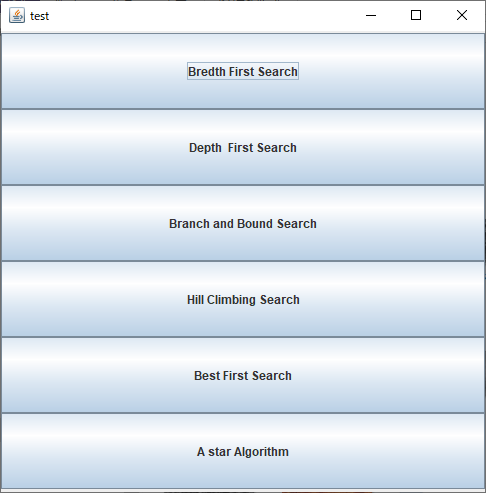
\includegraphics[bb=0 0 487 493,width=0.6\linewidth]{gui1.png}
  \caption{探索方法の選択}
  \label{fig:gui1}
\end{figure}

この中から行いたい探索方法を選んでクリックする。探索が終わると次のようになる。


\begin{figure}[!hbt]
  \centering
  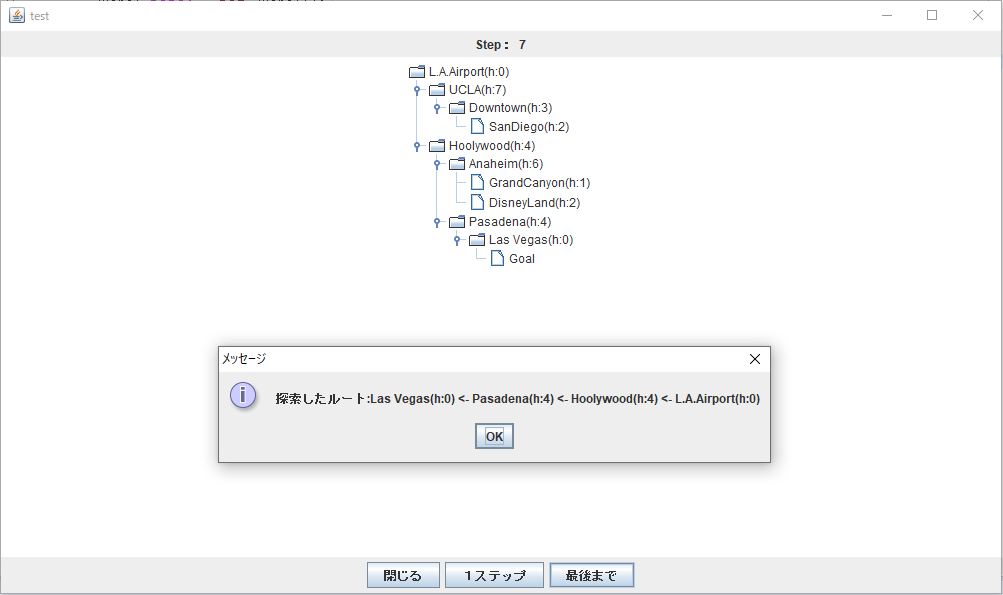
\includegraphics[bb=0 0 1003 595,width=1\linewidth]{gui2.png}
  \caption{探索終了}
  \label{fig:gui2}
\end{figure}
\subsection{考察}
今回の実装ではswingを使用してGUIを作成した。swingには、
ウィンドウや各種のボタンなどは取り揃えてあった。
しかし、元々描画をするためのものではないようなので、
図形を描画したり、レイアウトの位置を座標で指定したいときには
新しいクラスを作った方が良いと考えられる。この実装では、
レイアウトの方が間に合わなかったため、探索木はJTreeを利用した。

今回作ったGUIでは、1ステップごとに状況を確認できるように
1ステップごとに進む機能が実装されている。
この実装ではビジーウェイトなどを使わないようにするため、
スレッドを分けてwaitとnotifyで実現している。
それらは以下のように実装した。
\begin{lstlisting}[caption=wait部分,label=src:wait]
synchronized public void breadthFirst() {
  ...
  for (;;) {
    //1ステップごとに進むかどうか
    if (isStop) {
      try {
        wait();
      } catch (InterruptedException e) {
        // TODO 自動生成された catch ブロック
        e.printStackTrace();
      }
    }
  ...
}
\end{lstlisting}

\begin{lstlisting}[caption=notify部分,label=src:notify]
    ActionListener listener = new ActionListener() {

        //ボタンを押したときに呼ばれるメソッド
        @Override
        public void actionPerformed(ActionEvent e) {
            String cmd1 = e.getActionCommand();
            switch (cmd1) {
            //プログラムを終了する
            case "close":
                System.exit(0);
                break;
            //1ステップ進む
            case "step":
                synchronized (sh) {
                    sh.notifyAll();
                }
                break;
            //最後まで進む
            case "last":
                sh.isStop = false;
                synchronized (sh) {
                    sh.notifyAll();
                }
                break;
            default:
                break;
            }
        }
    };
\end{lstlisting}

waitやnotifyはObjectに対して働くため、Runnnableを作ってそこにSearchのメソッドを入れるという方法ではうまくいかなかった。
これはSearchのインスタンスとRunnnableのインスタンスが別であったために生じたことであると考えられる。
これを解決するため、SearchにRunnnableをimplementし、それをThreadの中に入れることによって、この問題を解決することができた。


\section{感想}
\subsection{}
  自分にとって、締め切りギリギリを攻めるのはいつものことであるが、
  グループワークとなると甚だ迷惑なので、
  しっかり時間をとって早めに済ませるようにしたい。グループ間の
  コミュニケーションについては、うまくアイスブレイク活動を行ったので
  話しやすい関係を築けた。
\subsection{}
 ほぼ初対面の人とのグループワークに慣れておらず、スムーズに課題を進めることができなかった。
  2か月という長くない時間だが、グループのみんなと仲良くなりたい。

% 参考文献
\begin{thebibliography}{99}
  \bibitem{text} 知能処理学の講義スライド、主に分枝限定法の部分
  \bibitem{goo} 矢印を描画 -JAVAで矢印を描画したいのですが、どうしたらいいのかわか- Java | 教えて!goo
  \url{https://oshiete.goo.ne.jp/qa/4014364.html} (2019年10月7日アクセス).
  \bibitem{swing} Swingを使ってみよう - Java GUIプログラミング
  \url{https://www.javadrive.jp/tutorial/} (2019年10月7日アクセス).
\end{thebibliography}

\end{document}
